\documentclass[aspectratio=169]{beamer}

\usepackage[russian]{babel}
\usepackage{amsfonts}
\usepackage{amsmath}
\usepackage{amssymb}
\usepackage[cp1251]{inputenc}
% \usepackage[utf8]{inputenc}
\usepackage{epigraph}
\usepackage{tikz}
\usepackage{xcolor}
\usepackage{verbatimbox}
\usepackage{pgfplots}
\pgfplotsset{width=10cm,height=6cm,compat=1.3}

\usepgflibrary{arrows}


\usetheme{Madrid}

\newcommand*{\sele}[1]{{\bf #1}}
\newcommand*{\sel}[1]{\textcolor{blue}{#1}}
\newcommand*{\prob}[1]{\textcolor{magenta}{#1}}
\newcommand*{\vs}[0]{\vspace{10pt}}
\newcommand<>{\fullsizegraphic}[1]{
%  \begin{textblock*}{0cm}(-1cm,-3.78cm)
  \includegraphics[width={\paperwidth}]{#1}
%  \end{textblock*}
}

\title[Technical Presentation]{Technical Presentation}
\author{Pavel Aitkulov}
\institute[]{ajtkulov@gmail.com}
\date{March 22, 2024}

\begin{document}


\frame{\titlepage}

\frame
{
\frametitle{About me}

\begin{itemize}
  \item software engineer
  \item scala, fp, reasonable fp
  \item chess, Elo = 2000..2100, max = 2118
  \item run, marathon: 3h 22m, $\frac{1}{2}$ marathon: 1h 38m, 10km: 40m 40s, 5km: 19m 48s
  \item billiard
  \item ChGK, What? Where? When?, team quiz
\end{itemize}


}


\frame
{
\frametitle{Agenda}

Best project?

\begin{itemize}
  \item most challenging
  \item biggest business impact
  \item rps, highload, etc
  \item social impact
  \pause
  \item \textbf{information gain}
\end{itemize}

\hspace{5pt}

\pause

It's about embeddings.
}

\frame
{
\frametitle{Spell checker}

Domain: company info, firmographics, B2B.
\vspace{5pt}

55-60M companies. 
\vspace{5pt}

We have a search API. Enhance your data in CRM. 
\vspace{5pt}

There are a lot of misspellings/typos in company names (human errors, legacy systems).
}



\frame
{
\frametitle{Spell checker, challenge}

Different languages, artificial names (Uber, Google, everyone wants to be unique).

\vspace{5pt}
\pause

\begin{itemize}
\item 9M unique words
\item 50M unique pairs
\item 65M unique triples
\end{itemize}

We don't want to drop long tail.

\vspace{5pt}
\pause

Frequencies: \textit{Apple INC $\rightarrow$ Aapple INC}, which one is more natural?
}


\frame
{
\frametitle{Spell checker, similarity}

Similar to auto-suggestion in Search Engine, in Word/Google Docs.
\vspace{5pt}

Specific domain. 

\vspace{5pt}

There are OSS solutions for 300K words, without frequencies.

\vspace{5pt}

Solr/Lucene/Elastic has its own solutions. Limited.

\vspace{5pt}
\pause
Natural language:
\begin{itemize}
\item 2-5K words daily
\item 50-200K vocabulary
\end{itemize}
}

\frame
{
\frametitle{Spell checker, input}

Company names, 55M.

\vspace{5pt}

API logs + output size, history, 6 months.

\vspace{5pt}

Every 15-17\% request contains a new word, that doesn't exist in the company's name set.

\vspace{5pt}

20-50\% of those queries could be fixed.

\vspace{5pt}

Depending on the client, we had a 20-30\% hit rate (precision).

}


\frame
{
\frametitle{Spell checker, typos types}

\begin{itemize}

\item Classic misspelling, insert/replace/delete.
\vspace{5pt}

\textit{
Carme Fresca Restaurante $\rightarrow$ Carne Fresca Restaurante}
\vspace{5pt}
\pause

\item 
Cut, last word: 

\textit{Carne Fresca Resta $\rightarrow$ Carne Fresca Restaurante}
\vspace{5pt}
\pause
\item
No spaces: \textit{carnefrescarestaurante $\rightarrow$ Carne Fresca Restaurante}
\end{itemize}
\vspace{5pt}
\pause
It is better to have context, at least 2 words.
\vspace{5pt}

\pause
Identification of error, based on freq. If $freq(word) \le 5\, ||\, freq(word_1\ word_2) \le f_2$.
\vspace{5pt}
}


\frame
{
\frametitle{Spell checker, Trie}

      \begin{figure}
        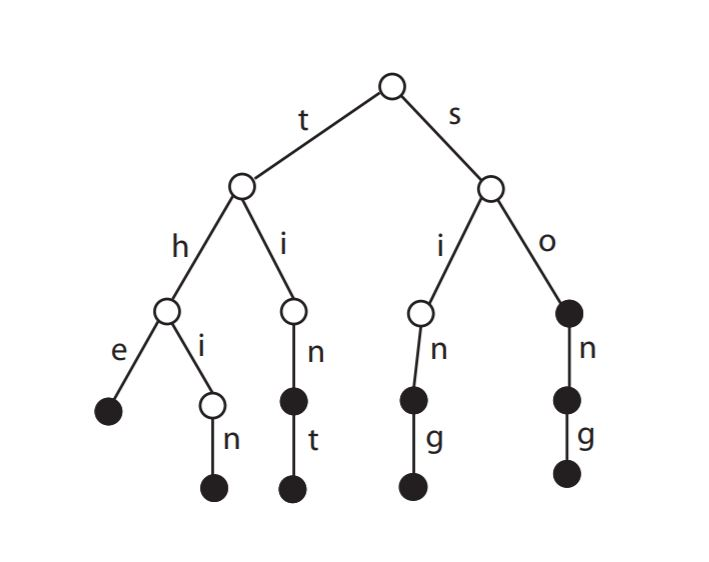
\includegraphics[height=0.3\textwidth]{trie.png}
      \end{figure}

\vspace{5pt}
\pause

Classic algorithm to fix Levenshtein-distance errors. Looking for \textit{sun}, \textit{son, sin} has 1 replacement, \textit{sing, song} has 1 replacement and 1 insert.

\vspace{5pt}
\pause

Compressed version. How do you store 9M unique and 50M pairs?
}


\frame
{
\frametitle{Spell checker, Bloom Filter}

      \begin{figure}
        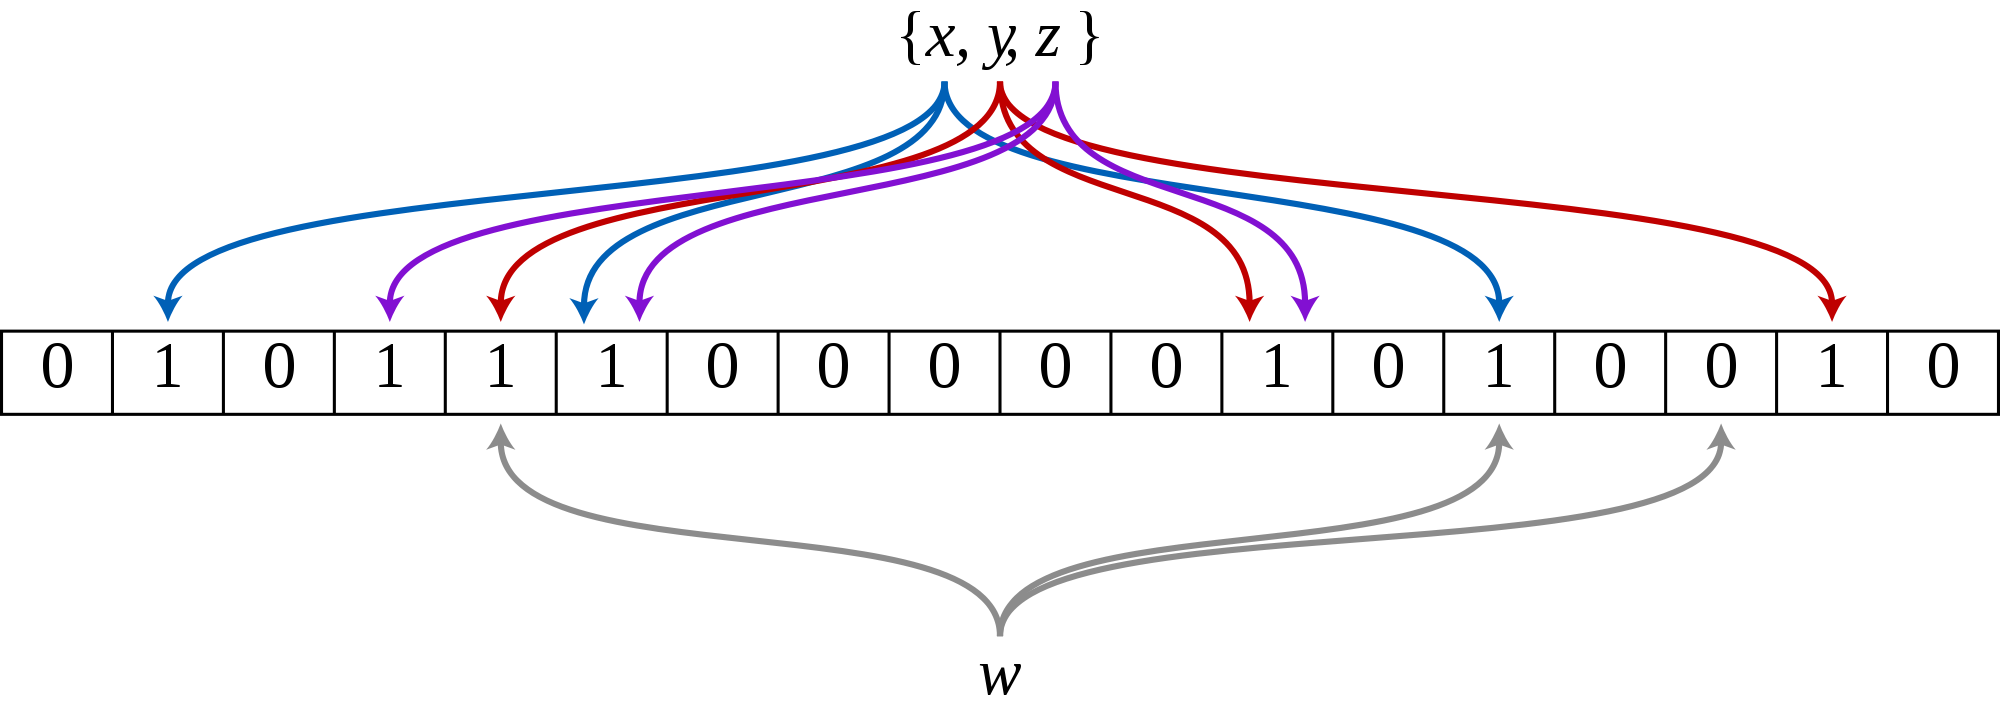
\includegraphics[height=0.3\textwidth]{bloom.png}
      \end{figure}

\vspace{5pt}
\pause

Compact HashTable (contains?), controlled FalsePositve-error, $10^{-6} \ldots 10^{-12}$, 10-30 bits per entity (1-3 bytes).

}

\frame
{
\frametitle{Spell checker, Trie as Bloom Filter}

Trie as interface:
\begin{itemize}
  \item contains a prefix
  \item contains a whole word, termination
  \item links to next level
\end{itemize}

\vspace{5pt}
\pause

Boolean queries = Two Bloom Filters.
\vspace{5pt}
\pause

Links to the next level = we have only 26 letters in English alphabet.

\vspace{5pt}

Optimization: use n-grams stats, there is no 'QZXP' in a dataset.
}

\frame {
\frametitle{Spell checker, Data Structures, Algorithms}

Trie as Bloom Filter. For 1-, 2-word ngrams. (actually, 3- was useless)
\vspace{5pt}

Frequencies as Count-Min-Sketch for 1-, 2-ngrams.

\vspace{15pt}
\pause

Levenshtein-distance errors. 
\vspace{5pt}

Cut and no-space tasks (a good task for interview).
  
\vspace{15pt}
\pause

We are trying to fix only 1 error, otherwise there are too many results.

\vspace{5pt}

Extra math to evaluate results. Smoothing. Get top-5 results.
\vspace{5pt}
\pause

$p(w_1 w_2 w_3 \ldots w_n) = p(w_1) \cdot p(w_2 | w_1) \cdot p(w_3 | w_1 w_2) \cdot \ldots p(w_n | w_1 w_2 \ldots w_{n - 1})$
$\approx p(w_1) \cdot p(w_2 | w_1) \cdot p(w_3 | w_2) \cdot \ldots p(w_n | w_{n - 1})$ 
}


\frame
{
\frametitle{Spell checker, final implementation}

Orb Intelligence, as a startup. 4-5 engineers, 1 ML person, 3 ML-interns, CEO, 1 sales, 1 team for ML markup.

\vspace{5pt}

Integration with Search API, python backend + Solr index (2 - 100 replicas).

\vspace{5pt}

Spell checker service, 1 instance, all indices in 20Gb RAM. Scala. 
\vspace{15pt}
\pause

Bloom Filter in Guava/Algebird is bad. Fork of addthis/stream-lib. CMS is enough.

Hit rate 20-30\%. With Spell checker we had an extra 3-5\% hit rate. 10-100 rps, max 4K.

\vspace{15pt}
\pause

One SE for 3-4 months, I'm. Plus, one SE for 1-2 weeks for integration, logs + analytics. In 2020.

}

\frame
{
\frametitle{Spell checker, outcome}


\begin{center}
  \begin{tabular}{cc}
Idea & Business outcome\\

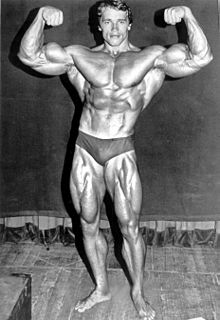
\includegraphics[height=0.2\textwidth]{arnold.jpeg} &
        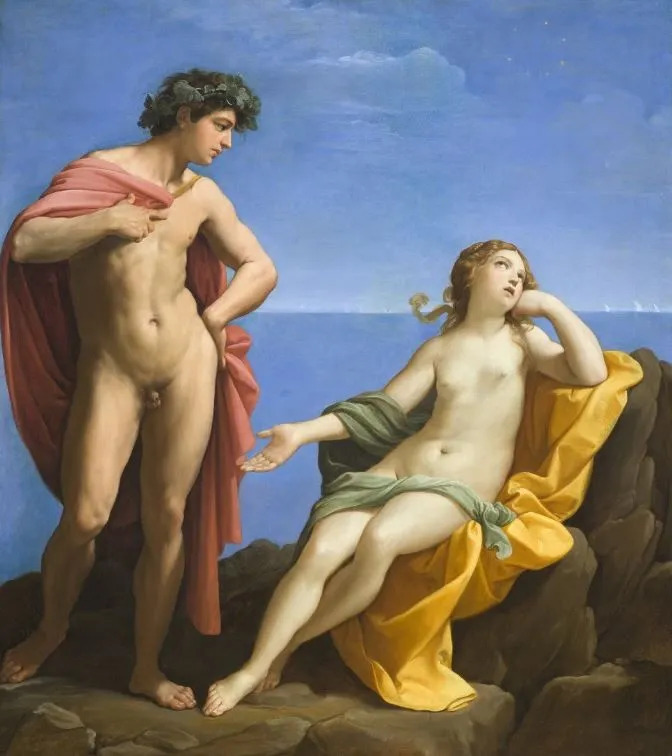
\includegraphics[height=0.2\textwidth]{ariadna.jpg}
  \end{tabular}
 \end{center}

\vspace{5pt}
\pause

Acquisition by Dun and Bradstreet. 

\vspace{5pt}

Search API was deprecated and shut down in 9 months later.

\vspace{5pt}
\pause

Trie as Bloom Filter. My personal idea, re-invented, there is an article from 2016 in bioinformatics with the same idea.
}




\frame
{
\frametitle{Duplicates detection}

Dun and Bradstreet, B2B, 600M companies profiles.

\vspace{5pt}
We want to find similar profiles.

\vspace{5pt}
Company name + full address (address1, address2, city, state, country, with empty value).

\pause
\vspace{15pt}
\textit{Wendy Coffee, 16 Park Square, London, England} $\approx$ \textit{Wendy's Coffee, 16N Park Square, London, England}

\vspace{15pt}
\pause

Solution with $O(n^2)$ doesn't work.

}


\frame
{
\frametitle{Duplicates detection, Locality Sensitive Hashing}

Classic hashing, equality of hash (almost) leads to equality on objects. Int32/Int64.

\vspace{15pt}
\pause

Locality Sensitive Hashing (LSH). Family of methods.

\vspace{5pt}

$LSH(object) \rightarrow object_{simpler}$. Grid in multidimensional space, caps on a sphere, vector.

\vspace{5pt}

The similarity of LSH values leads to similarity in objects.

}



\frame
{
\frametitle{Duplicates detection, Locality Sensitive Hashing + MinHash}

Convert text into a soup of n-grams; 2-3-4-length tokens, not words.

\vspace{5pt}

Convert soup of n-gram to binary vector via MinHash.

\vspace{5pt}

For each binary vector find all similar (by Hamming distance) vectors. See next slides
}

\begin{frame}[fragile]
\frametitle{Duplicates detection, MinHash - 2}
\begin{verbatim}
hashSet = ngrams.map(hash_function)

for idx in 0 until vector_size:
   permutation = genRandomPermutation(idx)
   output(idx) = min(permutation(hash_set))

\end{verbatim}

\vspace{5pt}

Output: Array[Integer]

\vspace{5pt}

Number theory, permutation is defined by $(a, b): f(x) = a \cdot x + b\, mod\, 2^{32}$.
Only $a$ is enough. We can apply $f^{-1}(x)$, doesn't matter.

\vspace{5pt}

Output: Array[Bit]. Apply $(x \rightarrow x\, mod\, 2)$


\vspace{15pt}

Reference: Mining of Massive Datasets
Jure Leskovec, Anand Rajaraman, Jeff Ullman
\end{frame}

\frame
{
\frametitle{Duplicates detection, ANN on binary vectors}

Hamming Distance = Levenshtein Distance with replacement.

\vspace{5pt}

We solved it with Trie as Bloom Filter in the previous task.

\vspace{5pt}

The tricky part: binary vector + ID encoding.

}

\frame
{
\frametitle{Duplicates detection, KNN}

Any solution with FAISS, HNSW, etc still works. 
\vspace{15pt}

Pros/cons, no graphs, less memory, 20-30 bytes per item.
}


\frame
{
\frametitle{Duplicates detection, implementation details}

600M company profiles, business registration name, brand name, multiple addresses. In total around 800M profiles.
\vspace{15pt}

Build index for all profiles. Traverse all other profiles against this index.
\vspace{15pt}

Index - 20Gb RAM.
\vspace{15pt}

24 nodes (32 GB RAM, 16 cpu), 1 week, Kafka for message bus, plain Scala. 
}


\frame
{
\frametitle{Duplicates detection, results}
\begin{center}
  \begin{tabular}{cc}
Idea & Business outcome\\

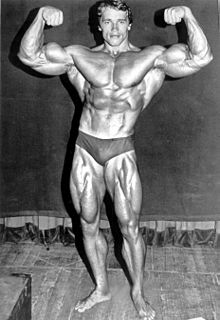
\includegraphics[height=0.2\textwidth]{arnold.jpeg} &
        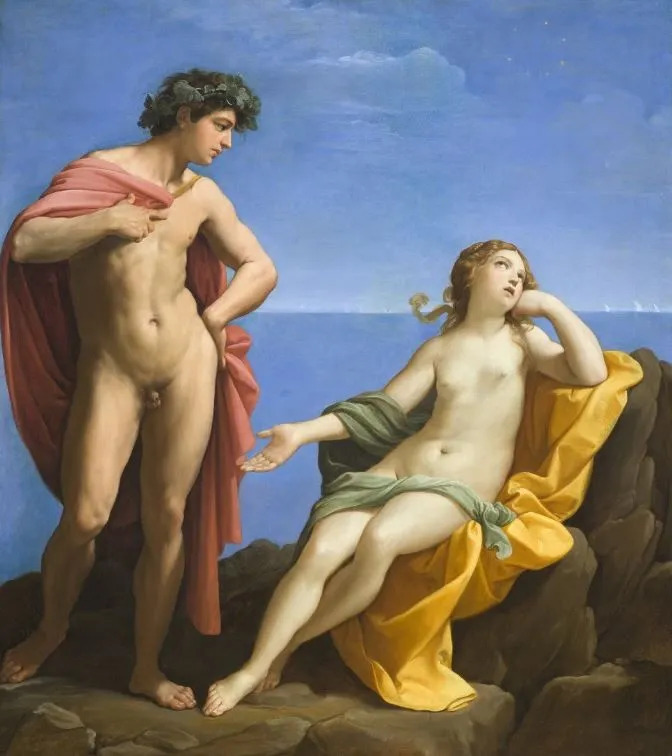
\includegraphics[height=0.2\textwidth]{ariadna.jpg}
  \end{tabular}
 \end{center}

\vspace{5pt}
\pause

6M similar profiles with different Hamming distance. To manually review, merge, or delete.
\vspace{5pt}


4M equal profiles, mostly, size 2 or 3. What went wrong: cluster 100K, should be preprocessed. $O(n^2)$ output. Duplicates could be automatically merged or deleted.

\vspace{5pt}

PoC state, one-off.
}


\frame
{
\frametitle{Dissernet}

Dissernet is a volunteer project dedicated to the verification of research articles and Ph.D. theses, focusing on detecting plagiarism and data manipulation.

\vspace{5pt}


\href{https://www.dissernet.org/}{https://www.dissernet.org/}

\vspace{5pt}

\href{https://en.wikipedia.org/wiki/Dissernet}{https://en.wikipedia.org/wiki/Dissernet}

}


\frame
{
\frametitle{Dissernet, what we do}

\begin{itemize}
\item Examination for text plagiarism
\item scrutiny of data plagiarism
\item detection of data manipulation
\item identification of reference manipulation
\item translation scrutiny from other languages
\end{itemize}
}


\frame
{
\frametitle{Dissernet, example}

      \begin{figure}
        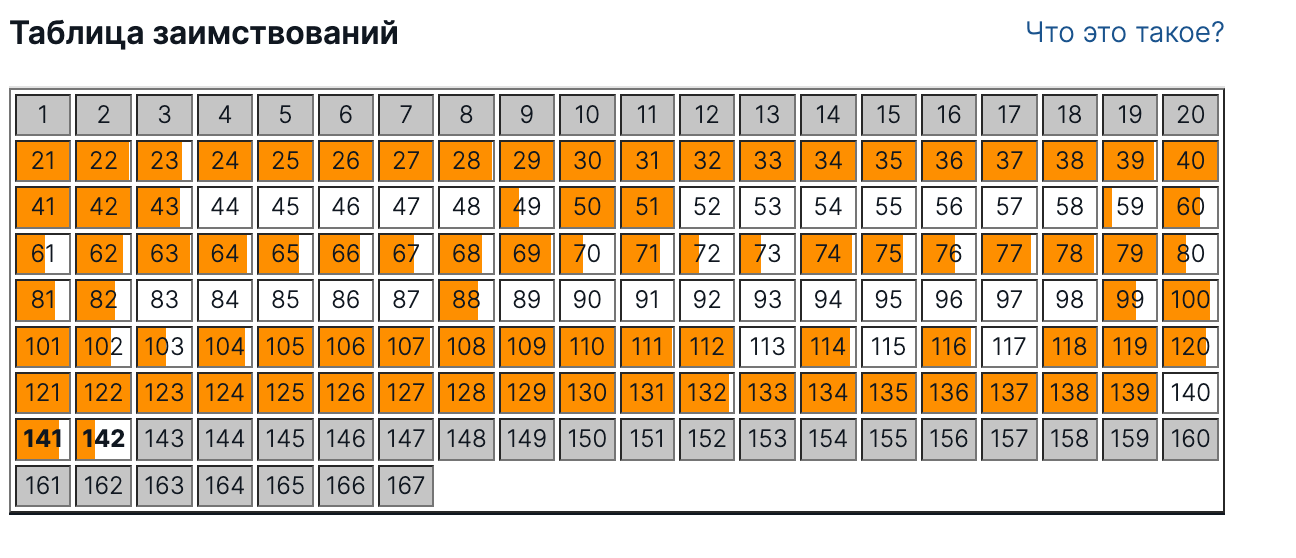
\includegraphics[height=0.3\textwidth]{diss1.png}
      \end{figure}


}

\frame
{
\frametitle{Dissernet, example}

      \begin{figure}
        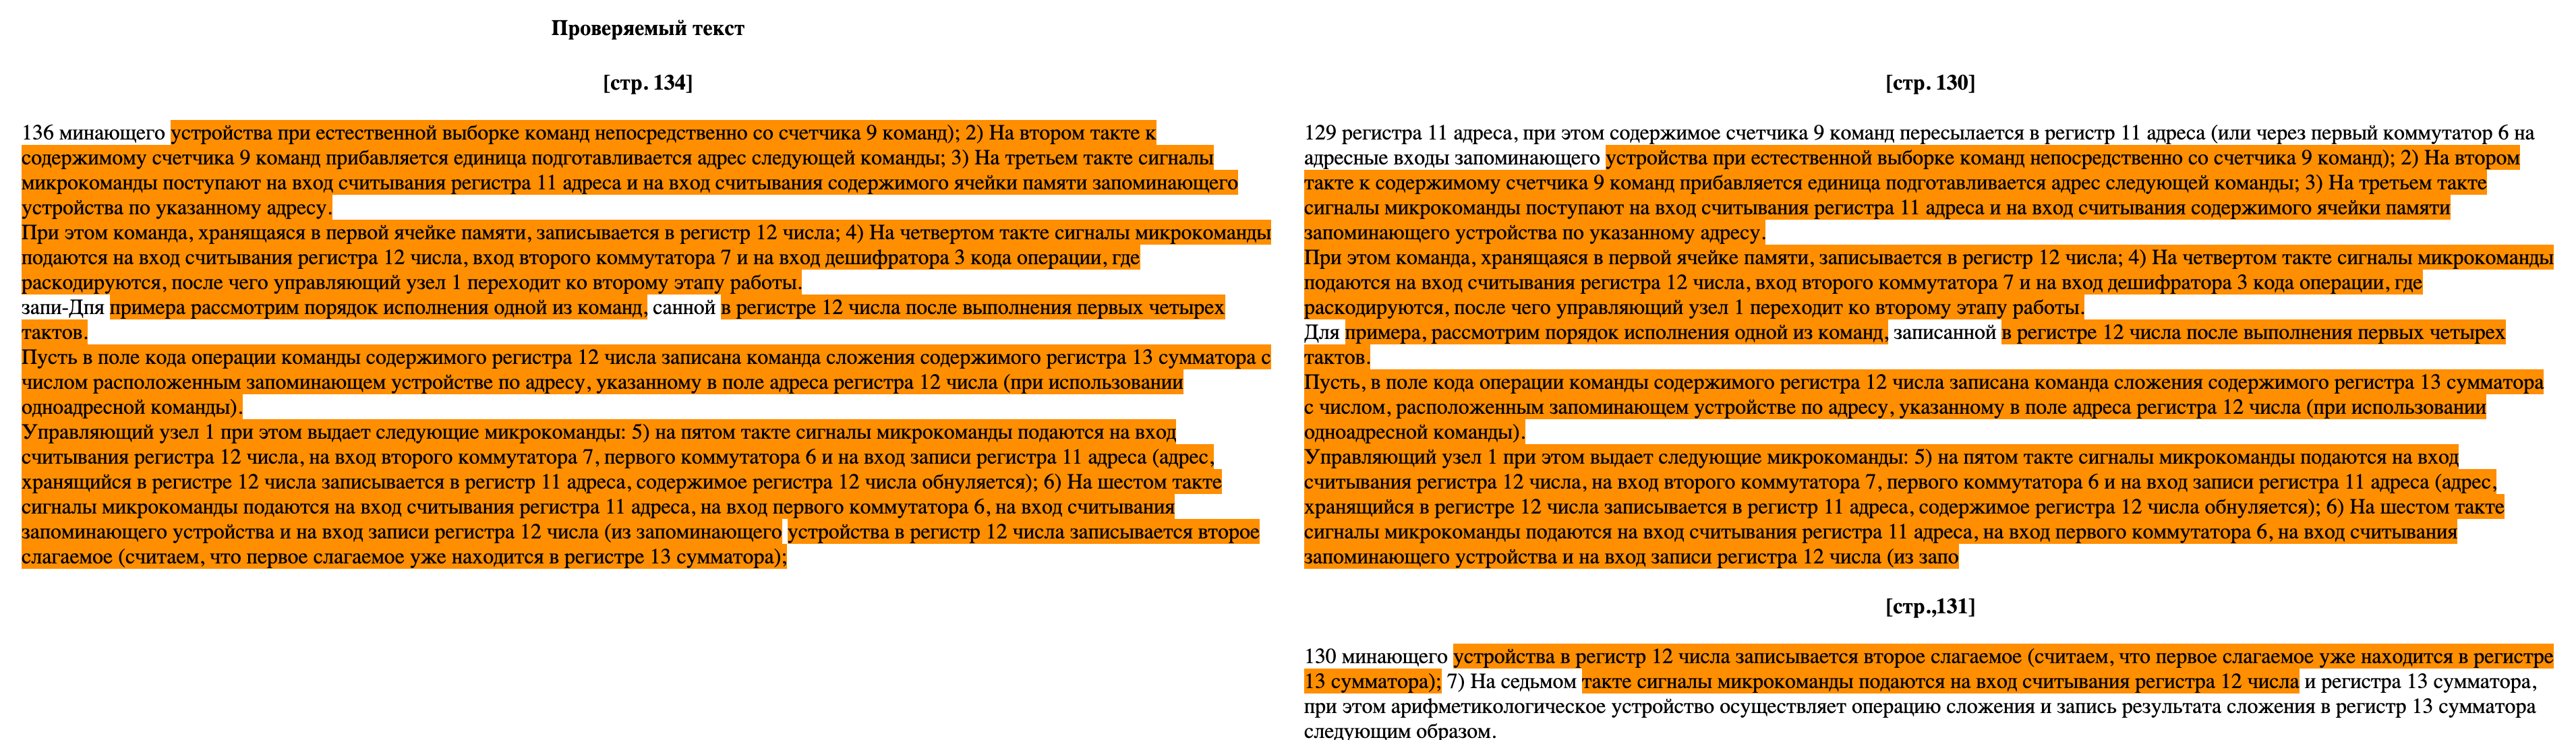
\includegraphics[height=0.3\textwidth]{diss2.png}
      \end{figure}
}

\frame
{
\frametitle{Dissernet, example}

      \begin{figure}
        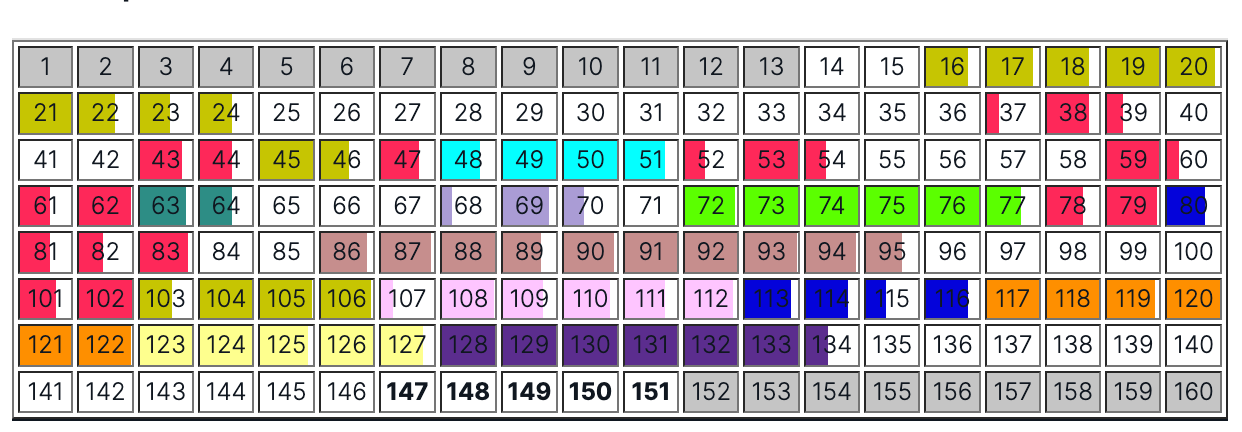
\includegraphics[height=0.3\textwidth]{diss4.png}
      \end{figure}
}


\frame
{
\frametitle{Dissernet, example}

      \begin{figure}
        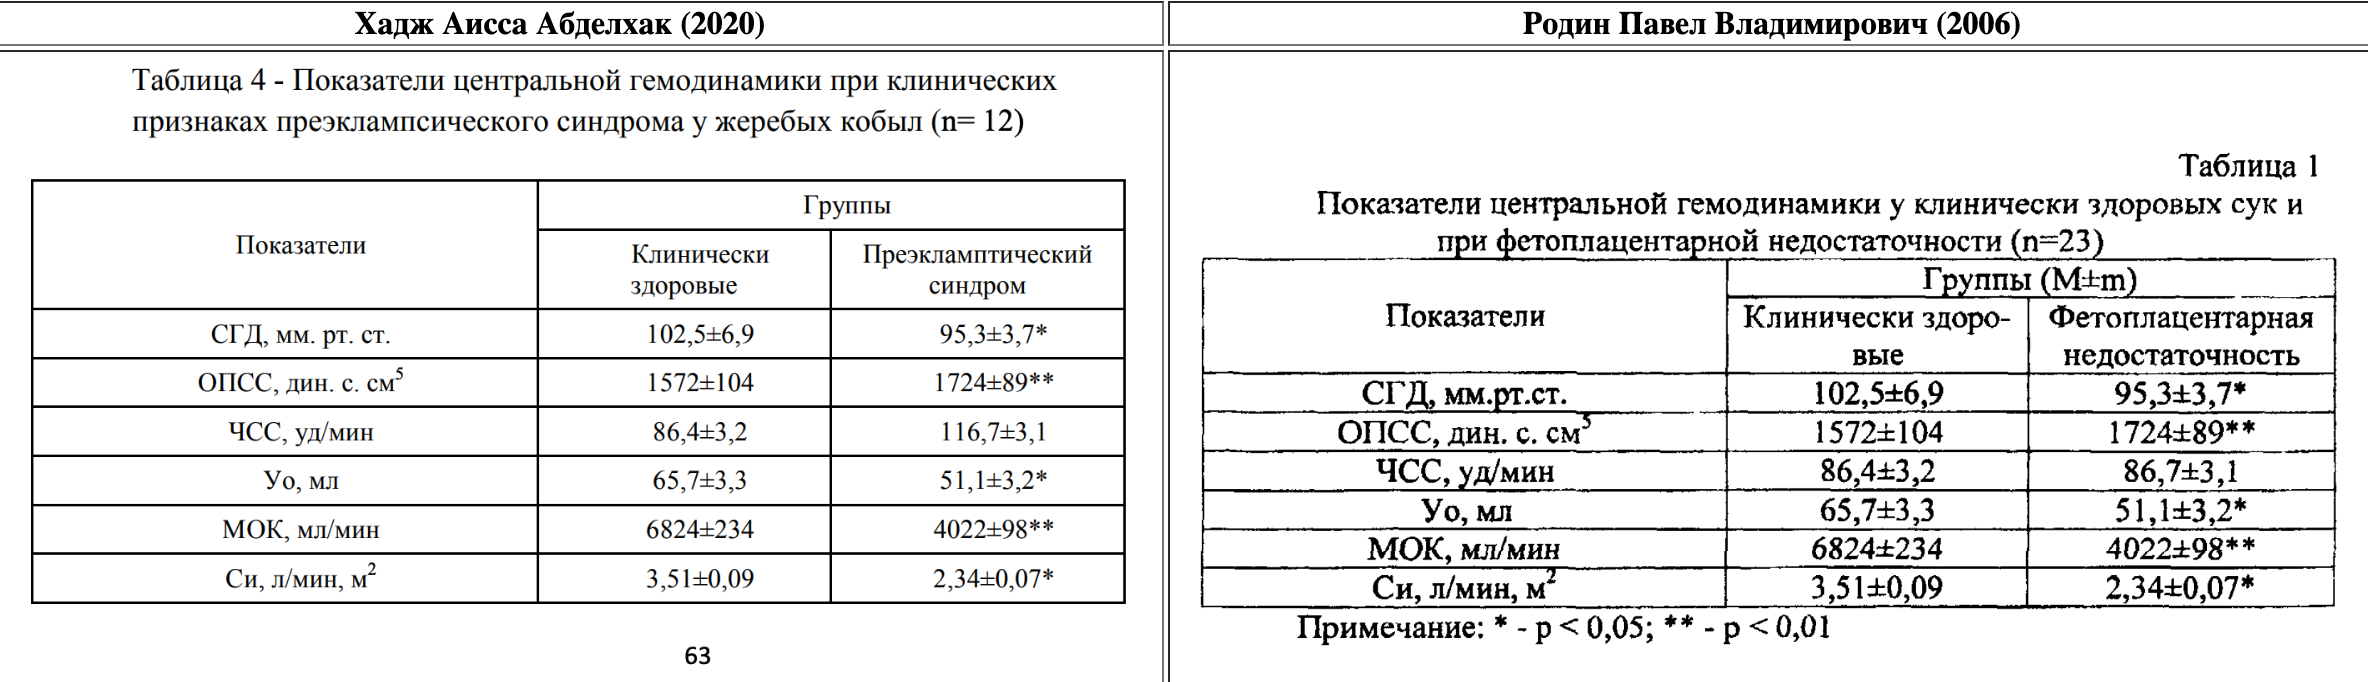
\includegraphics[height=0.3\textwidth]{diss3.png}
      \end{figure}
}


\frame
{
\frametitle{Dissernet, results}

\begin{itemize}

\item retraction of over 1400 Ph.D. diplomas
\item inclusion of 12K Ph.D. works and over 50K research articles in our comprehensive database

\end{itemize}
}

\frame {
  \frametitle{Dissernet, PhD cases}

  \begin{tikzpicture}

  \pgfplotstableread[row sep=\\,col sep=&]{
    interval  & allE & allT \\
    1995      & 1    & 1 \\
    1996      & 4    & 5 \\
    1997      & 3    & 4 \\
    1998      & 8    & 10 \\
    1999      & 72   & 86 \\
    2000      & 124  & 155 \\
    2001      & 132  & 155 \\
    2002      & 256  & 315 \\
    2003      & 438  & 499 \\
    2004      & 806  & 864 \\
    2005      & 942  & 1005 \\
    2006      & 1255 & 1350 \\
    2007      & 1033 & 1144 \\
    2008      & 832  & 929 \\
    2009      & 985  & 1101 \\
    2010      & 864  & 991 \\
    2011      & 1436 & 1667 \\
    2012      & 812  & 1325 \\
    2013      & 184  & 388 \\
    2014      & 79   & 142 \\
    2015      & 53   & 102 \\
    2016      & 22   & 47 \\
    2017      & 13   & 31 \\
    2018      & 0    & 20 \\
    2019      & 0    & 16 \\
    2020      & 0    & 4 \\
    }\mydata

    \begin{axis}[
            ybar,
            bar width=.06cm,
            scaled y ticks=false,
            x tick label style = {font = \small, text width = 1.7cm, align = center, rotate = 70, anchor = north east},
            symbolic x coords={1995, 1996, 1997, 1998, 1999, 2000, 2001, 2002, 2003, 2004, 2005, 2006, 2007, 2008,
            2009, 2010, 2011, 2012, 2013, 2014, 2015, 2016, 2017, 2018, 2019, 2020},
            xtick=data,
            width=15cm, height=7cm
        ]
        \addplot table[x=interval,y=allE]{\mydata};
        \addplot table[x=interval,y=allT]{\mydata};
        \legend{Mar 2021, Aug 2022};
    \end{axis}
\end{tikzpicture}

}

\frame
{
\frametitle{Dissernet}


\begin{center}
  \begin{tabular}{cc}
Social impact & Tech challenge\\

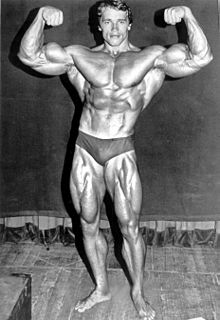
\includegraphics[height=0.2\textwidth]{arnold.jpeg} &
        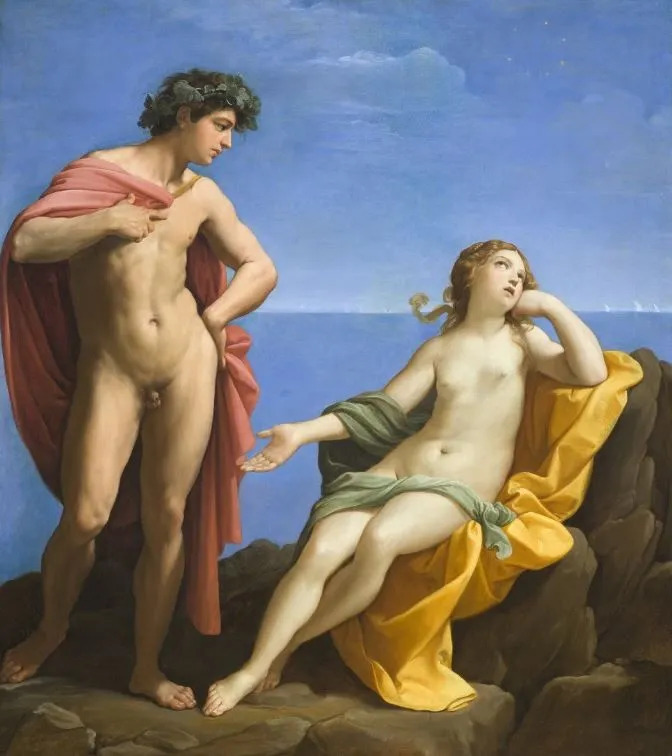
\includegraphics[height=0.2\textwidth]{ariadna.jpg}
  \end{tabular}
 \end{center}

\vspace{15pt}
\pause

Plain Scala. n-grams analysis, 500Gb of raw text, 2.6M articles, 600K dissertations.

\vspace{15pt}
\pause

Good task for interview.

}


\frame
{
\frametitle{QA}

      \begin{figure}
        
\includegraphics[height=0.46\textwidth]{folks.png}
      \end{figure}


}




\end{document}


